\documentclass[a4paper,10pt]{scrartcl}
\usepackage[german]{babel}
\usepackage{libertine}

\title{}
\author{Verkehrskonzept Nordkiez}

\begin{document}

\maketitle

\begin{abstract}
Dieses Konzept legt zwei Oberziele für die Entwicklung des Verkehrs im Nordkiez fest und macht 4 Implementierungsvorschläge.
\end{abstract}

\section{Hintergrund}
Im Nordkiez hat die Verkehrsbelastung zugenommen. Besonders in Nord-Süd-Richtung werden die Straßen als Schleichwege verwendet. Hierbei wird regelmäßig die Höchstgeschwindigkeit von 30 km/h erheblich überschritten. Dadurch ist es wiederholt zu Unfällen mit Personenschäden gekommen. 

Weiterhin verwendet auch der Lieferverkehr für das Gewerbegebiet am alten Schlachthof die Wohnstraßen des Nordkiezes als Abkürzung, die dafür nicht ausgelegt sind. Auch hier sind neben der allgemein vorhandenen Lärmbelastung des LKW-Verkehrs   Geschwindigkeitsüberschreitungen die Regel.

\section{Ziele}
Es werden für die Verkehrsentwicklung zwei Ziele festgelegt:
\begin{enumerate}
 \item Verringerung des Durchgangsverkehrs, insbesondere in Nord-Süd-Richtung 
 \item Umlenkung des Schwerlastverkehrs auf entsprechend gewidmete und ertüchtigte Straßen (Proskauer Straße, Möllendorfstraße, Eldenaer Straße)
\end{enumerate}


\section{Umsetzungvorschläge}
Zur Umsetzung der Ziele sind verschiedene Strategien denkbar. Die folgenden Strategien werden in diesem Konzept besprochen:
\begin{enumerate}
 \item Huckel 
 \item Einbahnstraßen 
 \item Straßensperren
 \item Plätze
\end{enumerate}

Als Gütekriterien werden herangezogen:

\begin{itemize}
 \item Effektivität
 \item Verträglichkeit mit Bedürfnissen der Anwohnenden
 \item Auswirkungen auf Zufahrten für Krankenwagen, Feuerwehr, Polizei, Müllabfuhr
 \item Preis 
 \item Dauer der Umsetzung 
\end{itemize}

Effektivität misst, inwieweit der Verkehr tatsächlich verringert wird. Bei den Bedürfnissen der Anwohnenden ist z.\,B. der Parksuchverkehr zu nennen. Die weiteren Kriterien sind intuitiv verständlich. Bei den Kosten werden nur Materialien aufgeführt, aber keine Planungs- oder Rechtskosten.

\newpage 
\subsection{Huckel}
Um die Einhaltung der Höchstgeschwindigkeit zu erreichen, werden insgesamt ca. 12 Huckel eingebaut. Die folgende Karte gibt einen Überblick  

\begin{figure}[h]
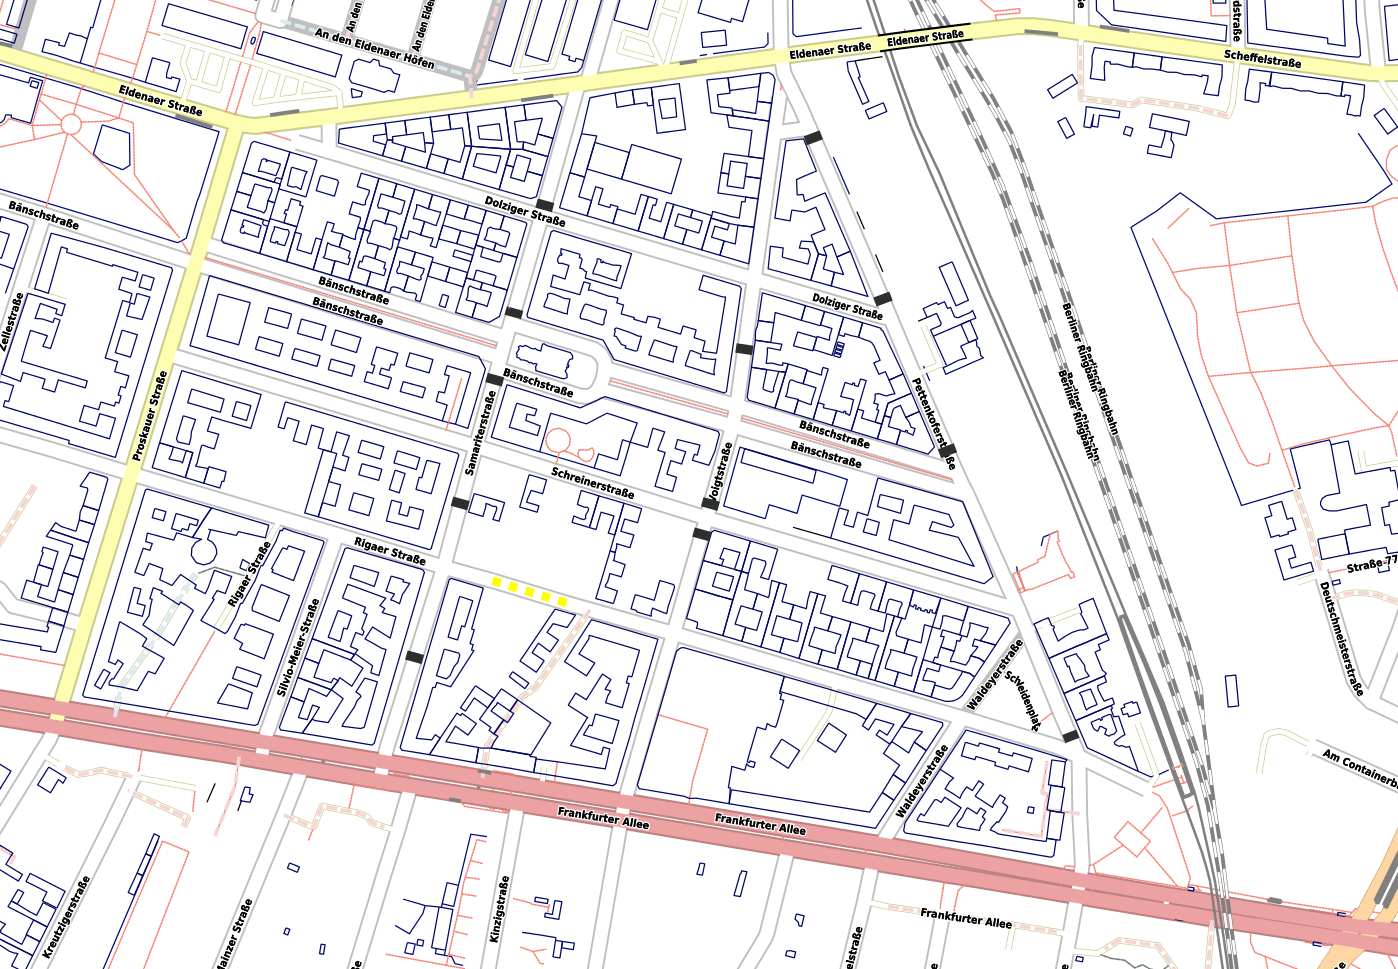
\includegraphics[width=\textwidth]{huckel.png}
\caption{Huckel}
\end{figure}

\begin{itemize}
 \item \textbf{Effektivität}: Verringerung der Geschwindigkeit ja, aber als Schleichweg eventuell immer noch attraktiv. Auswirkungen auf LKW unklar. 
 \item \textbf{Verträglichkeit}: gut
 \item \textbf{Auswirkungen auf Müllabfuhr etc}: unwesentlich
 \item \textbf{Kosten}: Huckel * 12 
 \item \textbf{Dauer}: unklar  
\end{itemize}
\newpage

\subsection{Einbahnstraßen}
Um den Kiez als Schleichweg unattraktiv zu machen, werden insgesamt 6 Straßenabschnitte neu als Einbahnstraßen ausgewiesen, wie in der Karte grün angegeben. (Bestehende Einbahnstraßen sind blau). Es ist weiterhin möglich, den Kiez von Norden nach Süden und von Süden nach Norden zu durchqueren. Dafür müssen jedoch Umwege in Kauf genommen werden. 

\begin{figure}[h]
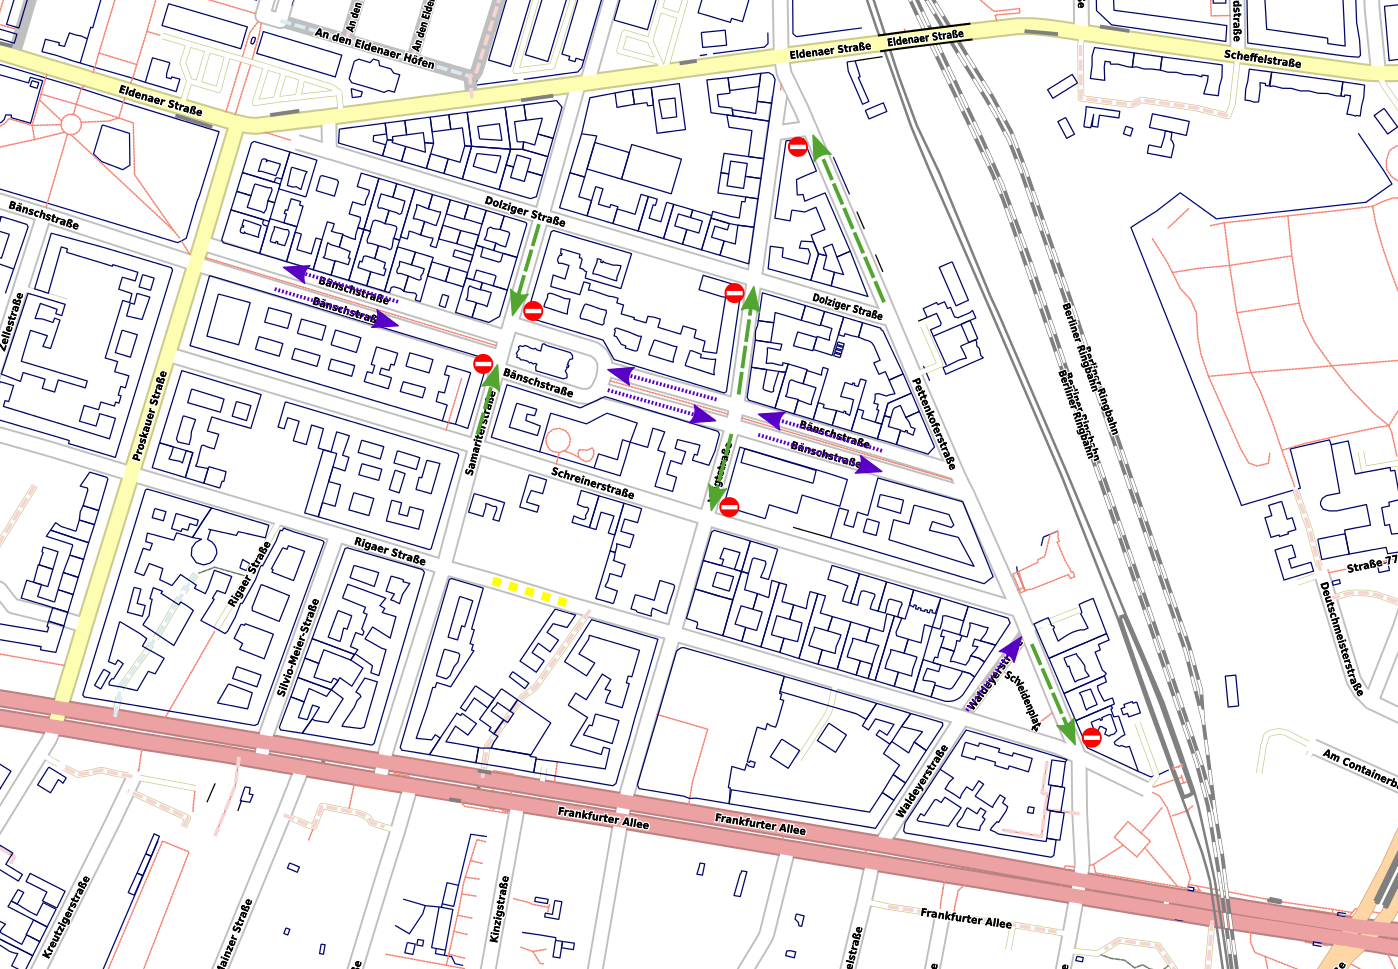
\includegraphics[width=\textwidth]{einbahnstrassen.png}
\caption{Einbahnstraßen}
\end{figure}

  
\begin{itemize}
 \item \textbf{Effektivität}: hoch
 \item \textbf{Verträglichkeit}: Eventuell längere Zufahrtswege für Anwohner und dadurch auch höhere Belastung der anderen Anwohnenden, aber weniger, als durch Durchgangsverkehr. 
 \item \textbf{Auswirkungen auf Müllabfuhr etc}: tbd
 \item \textbf{Kosten}: 6 Schilder {\glqq}Einbahnstraße{\grqq}; 6 Schilder  {\glqq}Einfahrt verboten{\grqq}	; 6 Schilder  {\glqq}Fahrräder frei{\grqq}. 
 \item \textbf{Dauer}: unklar  
\end{itemize}
\newpage
\subsection{Barrieren}
Die Samariterstraße, die Voigtstraße und die Pettenkoferstraße werden jeweils auf Höhe der Bänschstraße mit Metallbügeln für die Nord-Süd-Durchfahrt abgesperrt. Die Bügel werden mit reflektierenden rot-weißen Winkeln versehen. 


\begin{figure}[h]
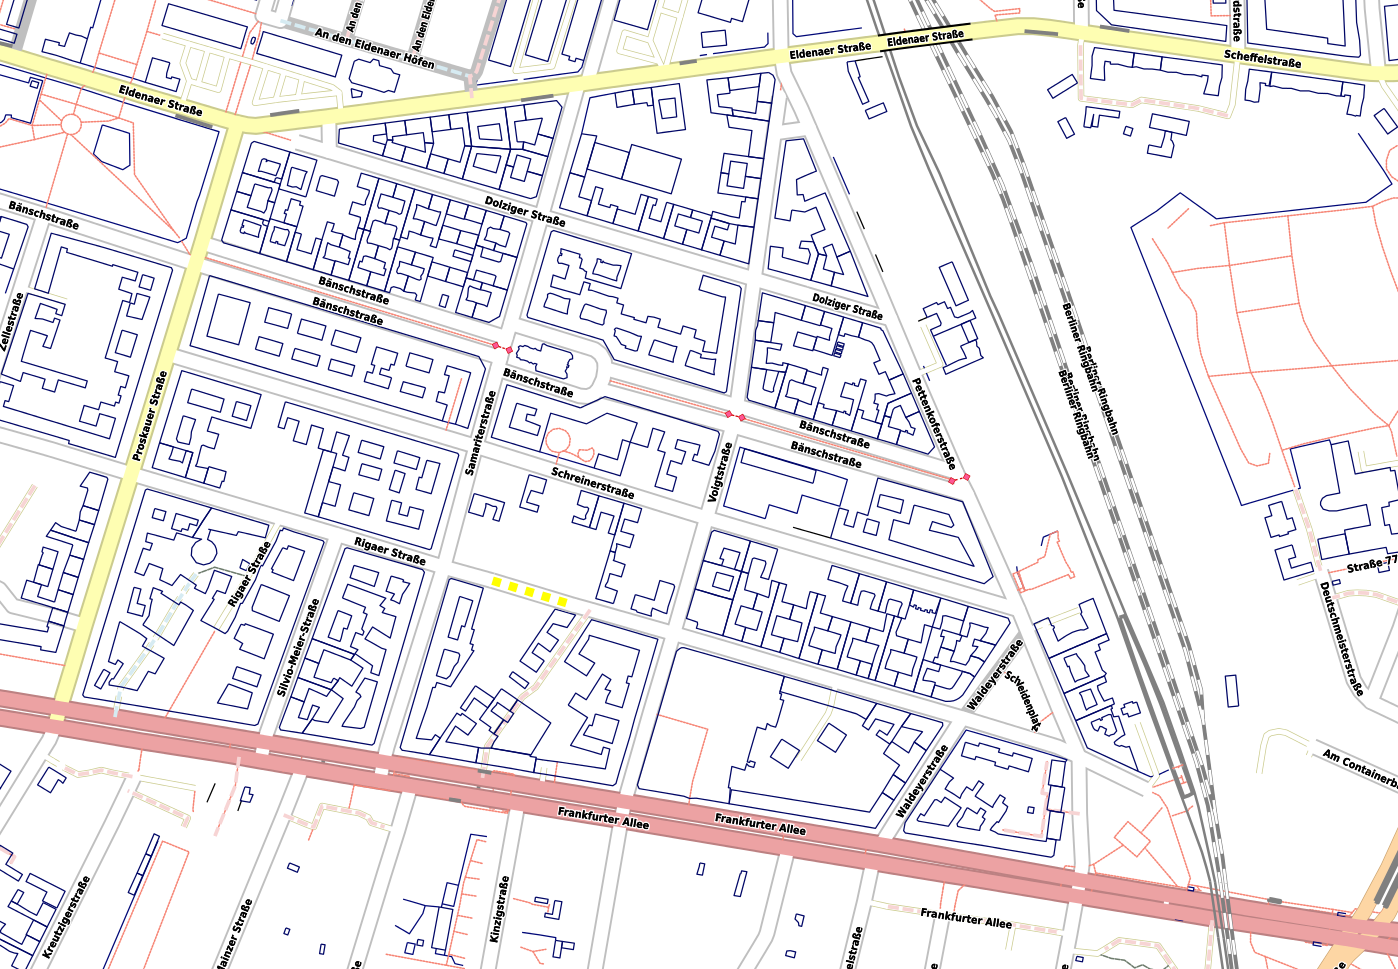
\includegraphics[width=\textwidth]{barriere.png}
\caption{Barrieren}
\end{figure}

\begin{itemize}
 \item \textbf{Effektivität}: hoch
 \item \textbf{Verträglichkeit}: Es ist nicht mehr möglich, vom Norden der Bänschstraße in den Süden zu gelangen. Der umgekehrte Weg ist um die Kirche herum möglich. 
 \item \textbf{Auswirkungen auf Müllabfuhr etc}: tbd
 \item \textbf{Kosten}: 6 Metallbügel mit Schildern
 \item \textbf{Dauer}: unklar  
\end{itemize}
\newpage
\subsection{Plätze}
Auf der Samariterstraße, der Voigtstraße und der Pettenkoferstraße werden jeweils auf Höhe der Bänschstraße kleine Plätze angelegt, die mit Bänken etc gestaltet werden. Ein Überfahren der Plätze ist für Autos nicht möglich, für Fahrräder hingegen schon. Funktional ist das Ergebnis identisch mit den Barrieren, ästhetisch sind die Plätze allerdings ansprechender.
 

\begin{figure}[h]
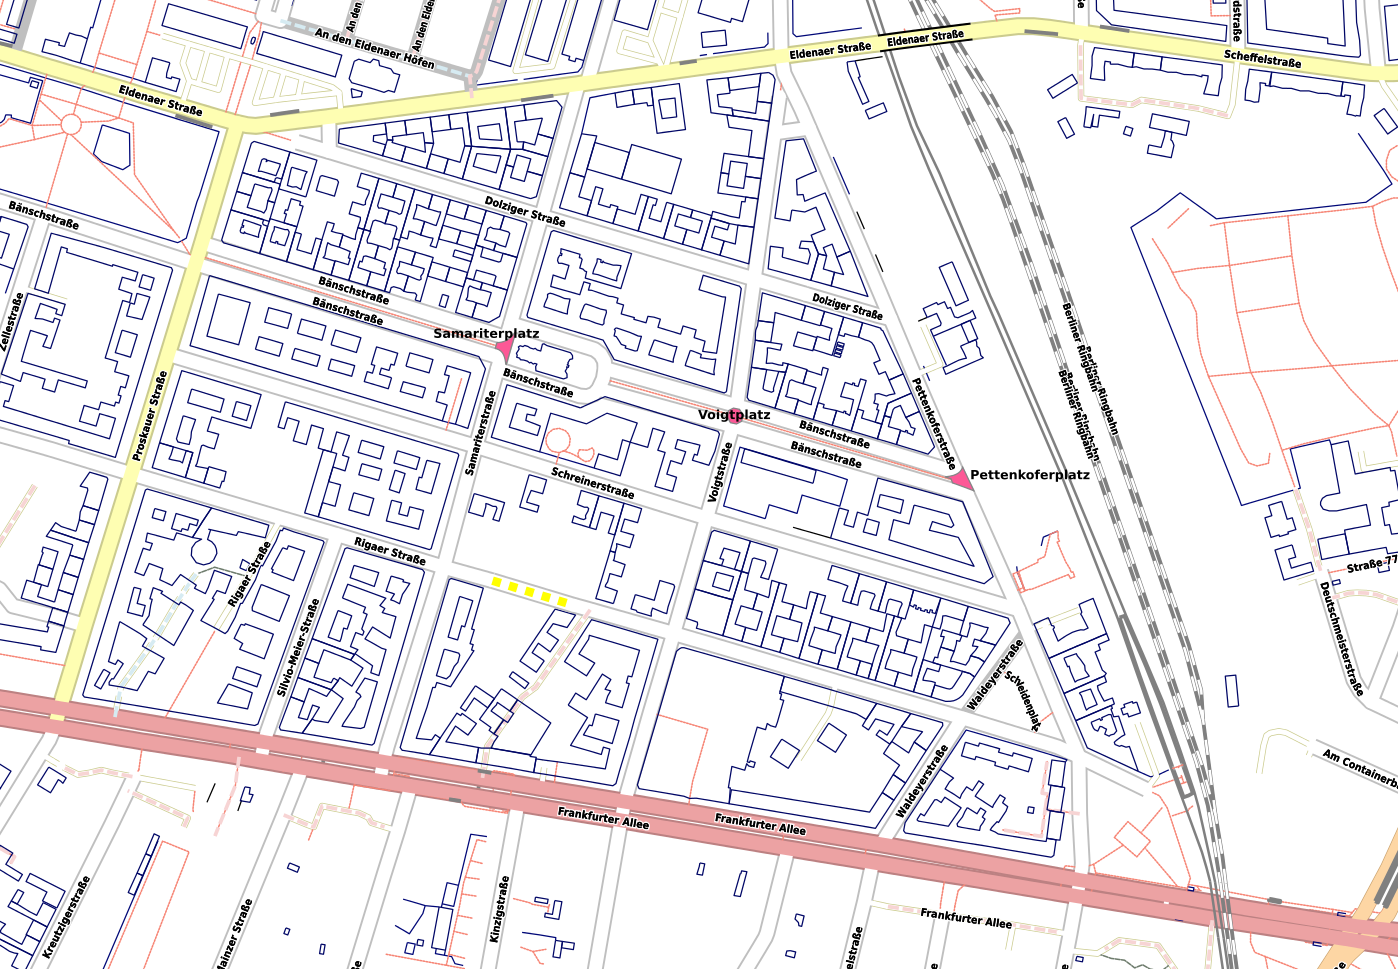
\includegraphics[width=\textwidth]{plaetze.png}
\caption{Plätze}
\end{figure}

\begin{itemize}
 \item \textbf{Effektivität}: hoch
 \item \textbf{Verträglichkeit}: Es ist nicht mehr möglich, vom Norden der Bänschstraße in den Süden zu gelangen. Der umgekehrte Weg ist um die Kirche herum möglich. 
 \item \textbf{Auswirkungen auf Müllabfuhr etc}: tbd
 \item \textbf{Kosten}: Änderung des Bodenbelages, Rinnstein etc, ggf weitergehende Gestaltung.
 \item \textbf{Dauer}: unklar  
\end{itemize}

\end{document}
